\chapter[Referencial Teórico]{Referencial Teórico} \label{chapter:Referencial Teórico}

Este capítulo apresenta conceitos da engenharia de software, de \textit{videogames} e de técnicas de matemática mental e interliga estes assuntos a fim de criar uma base teórica sólida para a realização deste trabalho, além de trazer ao leitor os conceitos necessários para o entendimento do mesmo.

\section{Jogos eletrônicos}
Para definir o que é um jogo eletrônico, ou um \textit{videogame}, como são mais popularmente conhecidos, primeiramente é necessário definir o que é um jogo. 

\citeonline{rogers_level_2010} define um jogo como uma atividade que requer no mínimo um jogador, tem regras e possui uma condição de vitória. Alguns exemplos simples de jogos que se encaixam nesta definição são: rebater uma bola na parede, arremessar um objeto o mais longe possível e memorizar a ordem de uma série de imagens.

\begin{citacao}
    Um \textit{videogame} é um modo de interação entre um jogador, uma máquina com um \textit{display} visual eletrônico, e possivelmente outros jogadores, que é mediada por meio de um contexto ficcional significativo para o jogador, e sustentada pelo apego emocional entre o jogador e os resultados de suas ações nesse contexto ficcional \cite[p.109 - 110, tradução nossa]{arjoranta_how_2019}.
\end{citacao}

O desenvolvimento de \textit{videogames} é um processo multidisciplinar, composto por pessoas das mais diversas áreas, como artistas, programadores e até advogados. 

A constante evolução da indústria de jogos faz com que conceitos importantes para a padronização de processos e produtos finais (os jogos) surjam. Uma análise mais profunda sobre os conceitos de teoria de jogos e de \textit{game design}, que são pilares para o entendimento deste trabalho, é de grande utilidade.

\subsection{Teoria de jogos}
A teoria de jogos é uma importante área da matemática que introduz ferramentas que tornam possível a análise de situações compostas por agentes que tomam decisões baseadas nas ações de outros agentes. 

\begin{citacao}
``A teoria de jogos pode também ser definida como o estudo sobre como o resultado final de uma situação competitiva é guiado pelas interações entre as pessoas envolvidas no jogo (também podem ser chamados de `jogadores' ou `agentes'), baseado nos objetivos e preferências desses jogadores e na estratégia adotada por cada um deles'' \cite[p.2, tradução nossa]{huang_game_2010}. 
\end{citacao}

Por estratégia entende-se apenas as diferentes maneiras, e por consequência, diferentes cadeias de ações que um agente pode adotar para alcançar um objetivo.

\subsection{Game Design}
Depois da popularização dos jogos eletrônicos como meio de entretenimento, a especialização da indústria em diferentes áreas deu-se de forma natural, visto que, com mais jogos sendo feitos, surge a necessidade de padronizar e evoluir todo o processo que permeia a produção de um \textit{game}. Segundo \citeonline{rogers_level_2010}, o profissional de \textit{game design} é responsável por criar as ideias e regras que compreendem o jogo, de modo a tornar possíveis diferentes estratégias que possam ser utilizadas pelos jogadores em diferentes partes do jogo. ``Quando pessoas jogam, elas têm uma experiência. O designer se importa justamente com essa experiência. Sem a experiência, o jogo não tem valor.'' \cite[p.10, tradução nossa]{schell_art_2008}. 


A área de \textit{game design} se trata exclusivamente da experiência do jogador dentro do \textit{game}, criando desde ambientes imersivos e interessantes para o jogador durante o ciclo completo do jogo.

\section{Engenharia de software aplicada a \textit{videogames}}
Segundo \citeonline{sommerville_software_2015}, a Engenharia de Software (ES) é uma disciplina da engenharia que está relacionada com todo o processo produtivo de um software, desde os estágios iniciais de especificação do sistema até a manutenção depois do início de seu uso. E, por meio da utilização de métodos, ferramentas e teorias, procura trazer manutenibilidade, confiabilidade, segurança, eficiência e aceitabilidade ao produto de software.

\begin{citacao}
``Videogames são produtos de software avançados, e, ao mesmo tempo, são produções complexas de criatividade e arte. Essa união de disciplinas, a necessidade de o produto ser divertido e o crescimento implacável da indústria de videogames, criaram diferenças significativas entre a engenharia de software tradicional e a engenharia de software para games (GSE)'' \cite[p. 1, tradução nossa]{chueca_consolidation_2024}.\footnote{``\textit{Video games are advanced software products and, at the same time, they are complex works of creativity and art [3]. This merge of disciplines, the need for the product to be fun, and the unrelenting growth of the video game industry have created significant differences between traditional Software Engineering (SE) and Game Software Engineering (GSE)}''}
\end{citacao}

Entretanto, vale lembrar que em alguns aspectos a engenharia de software tradicional e a engenharia de software para games (ou somente, engenharia de games) possuem similaridades significativas, de modo que a aplicação de conceitos, métodos e ferramentas da engenharia de software tradicional sejam inevitáveis.

\begin{figure}[h]
    \centering
    \caption{Imagem do \textit{game} Zelda: Tears of the kingdom}
    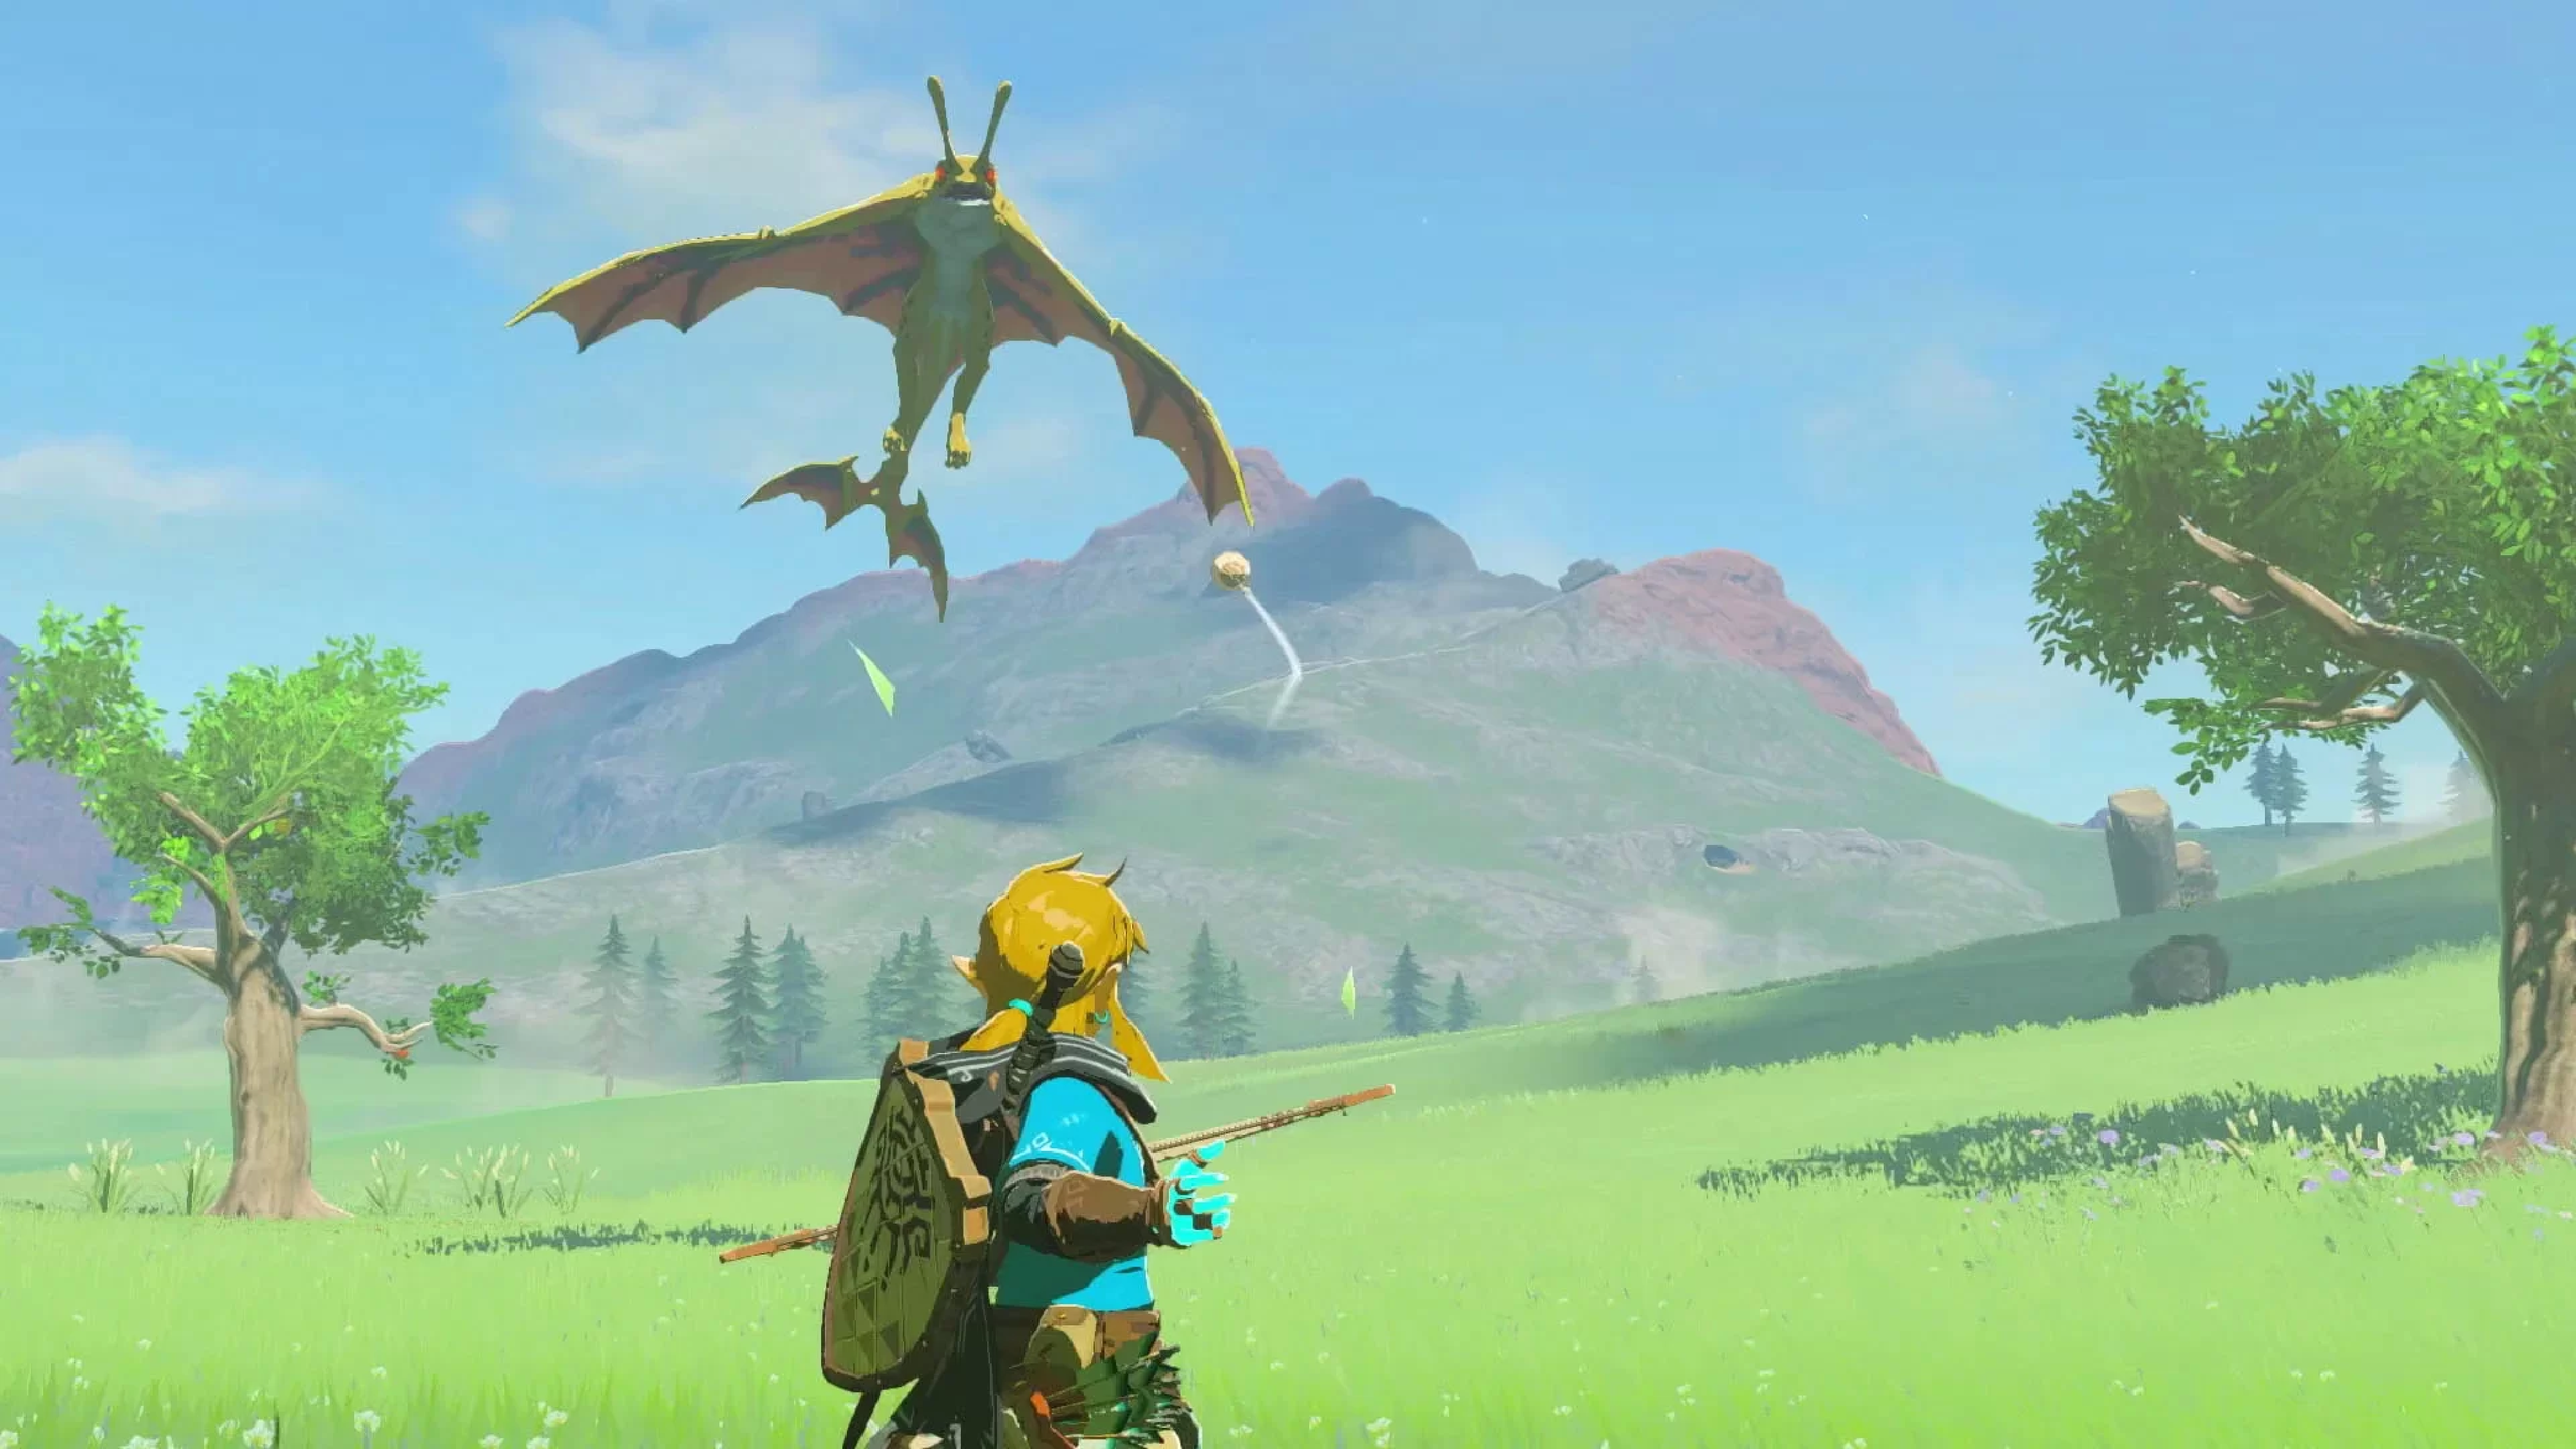
\includegraphics[width=320pt, keepaspectratio]{figuras/TearsOfTheKingdom.pdf}
    \label{fig:zelda_totk}
    \legend{Autor: Nintendo. Fonte: Google Imagens}
\end{figure}

Um dos aspectos dos quais a engenharia de games utiliza, apesar das diferenças, é a adoção de métodos de desenvolvimento de software. As metodologias se dividem em dois tipos, as metodologias tradicionais e as metodologias ágeis. No âmbito do desenvolvimento de games, as metodologias ágeis são preferencialmente adotadas, tendo em vista sua alta iteratividade e baixo foco na documentação, o que oferece facilidade ao time de desenvolvimento de um jogo para realizar atividades como o \textit{playtesting}, que consiste em realizar testes de versões específicas do jogo com jogadores selecionados para obter \textit{feedbacks} rápidos e corrigir erros e comportamentos indesejados antes do lançamento oficial.

No contexto de engenharia de games, é comum separar atividades com responsabilidades específicas para padronizar o processo e seguir o método de desenvolvimento escolhido pela equipe. Algumas das atividades comuns na engenharia de games são o levantamento de requisitos, o \textit{game design}, a implementação e o \textit{playtesting}.

No game Zelda: Breath of The Wild, os conceitos da GSE possibilitou a identificação de melhorias no game design durante sessões de \textit{playtesting}. As melhorias foram tão significativas que foram levadas como aprendizado para a criação do game que dá sequência à este, o \textit{Zelda: Tears of The Kingdom} (Figura \ref{fig:zelda_totk}).

\subsection{Levantamento de Requisitos}
``As pessoas e organizações têm desejos e necessidades de coisas a serem construídas ou de serem evoluídas. Chamamos essas necessidades de requisitos'' \cite[p. 9 - \textit{syllabus} do nível fundamental, CPRE]{ireb_downloads}. O objetivo da Engenharia de Requisitos (ER) é realizar o gerenciamento e o levantamento dos requisitos do sistema para que o usuário tenha suas necessidades e desejos realizados. A Figura \ref{fig:Processo Requisitos} descreve as etapas de uma iteração do processo de engenharia de requisitos.

\begin{figure}[h]
    \centering
    \caption{Processo de engenharia de requisitos}
    \includegraphics[width=320pt, keepaspectratio]{figuras/Requirements-truaduzido.pdf}
    \label{fig:Processo Requisitos}
    \legend{Autor: PNS (com adaptações). Fonte: Google Imagens}
\end{figure}

É comum realizar a utilização de técnicas que auxiliam no levantamento, priorização e gerenciamento dos requisitos de um projeto. Para a elicitação (levantamento) dos requisitos, podem ser utilizadas técnicas de coleta e técnicas geradora de ideias e desenhos.

\begin{citacao}
``As técnicas mais comuns utilizadas em elicitação de requisitos são as de introspecção, entrevista e análise de protocolos. A técnica de introspecção se baseia em imaginar que tipo de sistema eu iria querer se eu estivesse executando esta tarefa, utilizando este equipamento, entre outros. (...) As entrevistas podem ser divididas em entrevistas com questionários, entrevistas livres e grupos focais e de desenvolvimento de aplicações. (...) Já a técnica de análise de protocolos pede a um indivíduo que se envolva em uma tarefa, explicando ao mesmo tempo o seu processo de raciocínio'' \cite{andrade_de_moraes_utilizacao_2008}.
\end{citacao}

A escolha correta das técnicas de elicitação é fundamental para o sucesso de um projeto, visto que, caso os requisitos levantados estejam errados, o projeto não irá cumprir com as necessidades e vontades do usuário final. Para realizar a escolha correta, o tipo do sistema, o método de desenvolvimento de software, as pessoas envolvidas e a configuração organizacional devem ser levados em consideração.

Uma técnica de extrema importância é a priorização de requisitos, uma vez que em projetos de software devemos sempre levar em consideração o prazo dado, o tamanho da equipe e a capacitação da mesma para a execução de tarefas de desenvolvimento. Uma das técnicas mais difundidas entre os profissionais de engenharia de requisitos é a priorização MoSCoW, que consiste em separar os requisitos em diferentes categorias de priorização.

\begin{citacao}
    ``O nome \textit{MoSCoW} é derivado das primeiras letras dos critérios de priorização a seguir:
    
    \textit{Must have} (Mo),
    \textit{Should have} (S),
    \textit{Could have} (Co),
    \textit{Want to have but will not have this time round} (W).
    
    Para a maioria dos profissionais, ``W'' na verdade significa ``Won't have''. Técnicas de ranqueamento e técnicas de votação cumulativa são utilizadas para identificar as necessidades que precisam ser resolvidas, em oposição às necessidades das quais os \textit{stakeholders} gostariam que fossem resolvidas. Os casos de uso definidos para o sistema podem ser explicitamente associados com a necessidade resolvida por eles. Isso permite uma avaliação mais objetiva do benefício proporcionado por cada caso de uso e garante que cada caso de uso realmente esteja ajudando a sanar uma necessidade do \textit{stakeholder}.'' \cite[p.74]{bittner2003use}.
\end{citacao}

\subsection{Documento de \textit{Game Design}}
Segundo \citeonline{pedersen_game_2003}, o profissional de \textit{game design} é o visionário. É como o autor de um livro, que determinou o escopo e a descrição do produto com detalhes suficientes para que outros (o restante do time de desenvolvimento do game) possam entender e desenvolver o produto. Por esse motivo, uma das principais atribuições do \textit{game designer} dentro do time de desenvolvimento é ser o criador e escritor das ideias do \textit{game} em forma de um documento de \textit{game design}.

``O documento de \textit{game design} descreve tudo o que estará no jogo. É um documento muito importante que será consultado por toda a equipe durante a produção do jogo'' \cite[p. 72, tradução nossa]{rogers_level_2010}\footnote{\textit{``A GDD outlines everything that will be in the game. It’s a very important document that the entire team will refer to during the production of your game.''}} e, por isso, ele reflete detalhadamente a ideia do jogo, a arte, a trilha sonora, as mecânicas e até os diálogos entre os personagens existentes no game. Levando em consideração a necessidade do time de desenvolvimento, o tempo limite para a produção do game e o orçamento disponível, essa documentação pode tomar formas diferentes, desde um documento formal e padronizado até uma simples apresentação de \textit{slides}.

\subsection{Implementação}

\begin{citacao}
``O processo de desenvolvimento é algo que todo estúdio tem que seguir se ele quer criar um bom \textit{game}. Esse processo é iterativo, isso significa que algumas funcionalidades podem parecer boas quando escritas em papéis mas quando criadas não funcionam ou não são tão boas como esperado'' \cite[p. 10 tradução nossa]{tobar_carmona_game_2016}.\footnote{\textit{``The development process is something that every studio has to follow if they want to create a good game. This process is iterative, this means that some features could sound good when written in papers but then when created are not working properly or they are not as good as expected.''}}    
\end{citacao}

 Portanto, o processo de desenvolvimento é de extrema importância para a criação de bons \textit{games}, pois ela reflete diretamente o compromisso do time de desenvolvimento com a criação, o refino e a evolução do game. 

Dentro do processo de desenvolvimento, a implementação é a fase central, onde é feita a construção das ideias propostas nas fases de levantamento de requisitos e de \textit{game design}. É por meio dela que o \textit{game} toma forma para que a iteratividade do processo de desenvolvimento seja respeitada e também para que o maior número de erros e comportamentos indesejados sejam identificados e corrigidos antes de alcançar o jogador.

\subsection{\textit{Playtesting}}
``\textit{Playtesting} é simplesmente observar pessoas jogarem uma parte do jogo, por vezes com um questionário ou entrevista ao final. E depois usar o que você observa e escuta, para poder realizar mudanças no design do game'' \cite[tradução nossa]{gmtk_valves_secret_weapon}\footnote{\textit{``Playtesting is simply watching people play through a chunk of the game, sometimes with a questionnaire, or interview at the end. And then using what you see and hear to drive changes in the game's design.''}}. Segundo \citeonline{kim_swift_our-_journey_from_narbacular_drop_to_portal}, desenvolvedor da \textit{Valve} no game \textit{Portal} (Figura \ref{fig:Portal (valve)}), provavelmente, a coisa mais importante aprendida por ele foi o processo de realização de sessões de \textit{playtesting}.

\begin{figure}[h]
    \centering
    \caption{\textit{Game} Portal da Valve, em fase de \textit{playtesting}}
    \includegraphics[width=320pt, keepaspectratio]{figuras/PortalBeta.pdf}
    \label{fig:Portal (valve)}
    \legend{Autor: Valve. Fonte: Google Imagens}
\end{figure}

A fase de \textit{playtesting} precisa ser tratada como prioridade no desenvolvimento de um \textit{game}, pois nela são colhidos os principais \textit{feedbacks} sobre o comportamento atual e sobre o \textit{game design}. A aplicação de um questionário ou de uma entrevista direcionada ao final de uma sessão de \textit{playtesting} faz com que o time de desenvolvimento consiga colher respostas específicas para aplicar mudanças e melhorias no \textit{game}. 

Mas ainda assim, muitas respostas podem ser colhidas apenas observando o jogador durante a sessão de \textit{playtesting}. Dificuldades encontradas pelo jogador durante o \textit{game}, falhas na visualização de objetos cruciais à progressão, ou até a frustração passada por ele durante o game podem ser importantes para a realização de ajustes no design do jogo.

\section{Matemática mental} \label{section: matematica mental}
``É consenso,  entre  os  professores  da  educação  básica,  as  dificuldades enfrentadas ao ministrar aulas de matemática, não só pela complexidade dos conteúdos,  mas  também  pela  difícil  assimilação  de  conceitos  pelos  alunos'' \cite{nascimento_os_2023}. Segundo dados coletados pelo Instituto Nacional de Estudos e Pesquisas (INEP), por meio do Sistema de Avaliação do Ensino Básico (SAEB) 2021, 55,3\% dos alunos do ensino fundamental brasileiro pertencem aos 4 níveis inferiores de proficiência de matemática, do total de 8 níveis nos quais os alunos são avaliados.

Como apontado por \citeonline[tradução nossa]{benjamin_secrets_2006}, ``muitas vezes, a matemática é ensinada como um conjunto rígido de regras, deixando pouco espaço para pensamento criativo''\footnote{\textit{``Too often, math is taught as a set of rigid rules, leaving little room for creative thinking.''}}. Com isso, muitos alunos podem acabar sendo desmotivados e até pensar que habilidades matemáticas são inatas. Mas, como toda habilidade, ela pode ser aperfeiçoada e treinada por meio do aprendizado de técnicas facilitadoras. 

\begin{citacao}
    ``A base da Matemática é a aritmética.  Alicerçado na aritmética temos praticamente todos os  outros  conhecimentos  matemáticos.  Para  compreender  a  subtração,  é  necessário  primeiro, compreender bem a adição. Para compreender a multiplicação é necessário ter conhecimentos de   adição   e   subtração.   Da   mesma   forma,   para   compreender   a   divisão,   é   necessário conhecimentos de adição, subtração e multiplicação. Assim, para que o aluno  tenha um bom entendimento e uma boa relação com a Matemática, é imprescindível que ele saiba aritmética'' \cite{berticelli_aritmetica_2023}.
\end{citacao}

Diversas técnicas são ensinadas por \citeonline{benjamin_secrets_2006} no livro \textit{Secrets of mental Math: The Mathemagician's guide to lightning fast calculation and amazin math tricks}, com o objetivo de despertar o interesse e a curiosidade do leitor, para que, com as técnicas aprendidas, este possa não só impressionar amigos, familiares e colegas, mas também melhorar suas habilidades aritméticas. As principais técnicas apresentadas no livro que serão abordadas neste trabalho são a multiplicação instantânea, adição e subtração mental, multiplicação básica e divisão mental. Para melhor abstrair os conteúdos dos métodos ensinados, é necessário saber que o princípio fundamental da matemática mental é ter uma visão de resolução de problemas, transformando um problema grande em alguns outros problemas mais fáceis de serem solucionados.

\subsection{A multiplicação instantânea}
Uma das técnicas mais interessantes é a multiplicação de qualquer número de dois dígitos por 11. Assim que ela se torna conhecida, fica muito fácil realizar esse tipo de operação, dá a quem aprende a sensação de grande proficiência em matemática e causa grande admiração por parte de quem vê essa técnica sendo utilizada.

Utilizando as técnicas apresentadas por \citeonline{benjamin_secrets_2006}, para se multiplicar qualquer número de dois dígitos por 11, basta somar os dois dígitos, caso o resultado seja menor que 10, e colocar o resultando entre os dígitos originais, da seguinte forma:
\[32 \times 11\]
\[3 + 2 = \textbf{5}\]
\[32 \times 11  = 3\textbf{5}2\]


Agora, suponha que a soma dos dois dígitos seja maior que 10: como proceder? Nesse caso, devemos somar 1 ao primeiro dígito do número original, e colocar normalmente o segundo dígito entre os dígitos originais. Vejamos o exemplo abaixo:

\[85 \times 11\]
\[8 + 5 = \textbf{13}\]
\[85 \times 11 =  \textbf{93}5\]

Um outro exemplo seria: \begin{math} 57 \times 11 \end{math}. Como \begin{math} 5 + 7 = 12 \end{math}, o resultado é \begin{math} 627 \end{math}. Similarmente, uma conta muito comum é \begin{math} 99 \times 11\end{math}. Utilizando a técnica ensinada, podemos fazer: \begin{math} 9 + 9 = 18\end{math}, obtendo:

\begingroup
    \setlength{\tabcolsep}{0.5pt}
    \begin{center}
        \begin{tabular}{c c c c}
            & 1 & & \\
            & 9 & 8 & 9 \\
            \hline
            \textbf{1} & \textbf{0} & 8 & 9
        \end{tabular}
    \end{center}
\endgroup

Também é possível utilizar este método em números de três dígitos. Por exemplo, para o número 314, a resposta ainda começa com 3 e termina com 4. E, como \begin{math}3+1=\underline{\textbf{4}}\end{math} e \begin{math}1+4=\underline{\textbf{5}}\end{math}, o resultado é igual a \begin{math}3\underline{\textbf{45}}4\end{math}.

\subsection{A adição e subtração mental}
Utilizando a técnica de adição e subtração da esquerda para a direita, é possível realizar cálculos matemáticos mais rapidamente para uma grande variedade de números encontrados no dia a dia. 
\begin{citacao}
    ``Existem diversas boas razões pelas quais é melhor realizar cálculos matemáticos mentais pensando da esquerda para a direita. Afinal, nós fazemos a leitura de números da esquerda para a direita, pronunciamos seus nomes da esquerda para a direita, então, é simplesmente mais natural pensar (e realizar cálculos) da esquerda para a direita'' \footnote{\textit{``There are many good reasons why it is better to work from left to right. After all, you read numbers from left to right, you pronounce numbers from left to right, and so it’s just more natural to think about (and calculate) numbers from left to right.''}}\cite[p. 12, tradução nossa]{benjamin_secrets_2006}.
\end{citacao}

\subsubsection{Adição mental}

Os problemas de adição mais fáceis são os que não requerem que um número seja carregado para a outra casa (o ``vai um''). Por isso, o pensamento da esquerda para direita será demonstrado a partir deste problema simples até problemas mais complexos. Tomemos como exemplo a seguinte expressão: \begin{math}47 + \underline{\textbf{32}}\end{math}. Para dividir o problema em problemas menores, podemos escrever a mesma adição na forma \begin{math}47 + \underline{\textbf{30 + 2}}\end{math} e, por consequência, pensar da seguinte forma:

\begingroup
    \setlength{\tabcolsep}{0.5pt}
    \begin{center}
        \begin{tabular}{c c c}
            & \textbf{4} & 7 \\
            + & \textbf{3} & 0 \\
            \hline
            & \textbf{7} & 7 \\
        \end{tabular}
    \end{center}
\endgroup

Por fim, basta solucionar o problema mais simples (adicionar 2 ao resultado parcial) para obter o resultado final: 
\[7{\textcolor{blue}{\textbf{7}}} + \textcolor{blue}{\textbf{2}} = 7\textcolor{green!60!black}{\textbf{9}}\]

O diagrama a seguir exemplifica o processo de pensamento:

\begingroup
    \setlength{\tabcolsep}{0.5pt}
    \begin{tabular}{c c c c c}
         47 + 32 & = & 77 + 2 & = & 79 \\
         & (primeiro adicionar 30) & & (depois adicionar 2) & \\
    \end{tabular}
    \newline
\endgroup

Todo este processo pode ser utilizado para solucionar expressões matemáticas onde há a necessidade de que um número seja carregado para a próxima casa. Na prática, podemos tomar como exemplo a expressão \begin{math}67 + 28\end{math}. Utilizando um diagrama para representar o processo de pensamento, podemos solucionar a expressão da seguinte forma:

\begingroup
    \setlength{\tabcolsep}{0.5pt}
    \begin{tabular}{c c c c c}
         84 + 57 & = & 134 + 7 & = & 141 \\
         & (primeiro adicionar 50) & & (depois adicionar 7) & \\
    \end{tabular}
    \newline
\endgroup

Para realizar a adição de números de três dígitos, seguimos o mesmo processo de pensamento, realizando a divisão do problema original em problemas menores. Assim, podemos computar o resultado da adição \begin{math}538 + 327\end{math}. Usando o diagrama de processo mental, podemos executar o cálculo da seguinte maneira:

\begin{itemize}
    \item primeiro adicionar 300: \begin{math}\textcolor{blue}{\textbf{5}}38 + \textcolor{blue}{\textbf{3}}27 = \textcolor{green!60!black}{\textbf{8}}38 + 27\end{math}
    \item depois adicionar 20: \begin{math}8\textcolor{blue}{\textbf{3}}8 + \textcolor{blue}{\textbf{2}}7 = 8\textcolor{green!60!black}{\textbf{5}}8 + 7\end{math}
    \item por fim, adicionar 7: \begin{math}85\textcolor{blue}{\textbf{8}} + \textcolor{blue}{\textbf{7}} = 8\textcolor{green!60!black}{\textbf{65}}\end{math}
\end{itemize}

Todos os problemas de adição mental podem ser resolvidos desta maneira. Basta continuar dividindo o problema inicial em problemas menores, e solucionar cada um destes. Quando realizamos essa divisão em pequenos problemas, primeiramente é recomendado que os dados sejam ditos em voz alta e depois, com a prática, realizar a solução deles mentalmente. O fato de registrarmos mentalmente os resultados das operações, nos dispensa a necessidade de memorizar o ``vai um'' para soma-lo ao resultado final.

\subsubsection{Subtração mental}
Para realizar subtrações, os mesmos princípios e técnicas serão utilizados para facilitar o desenvolvimento e a resolução de expressões. Um problema simples seria:

\begingroup
    \setlength{\tabcolsep}{0.5pt}
    \begin{center}
        \begin{tabular}{c c c c}
            & 8 & 5 & \\
            - & 2 & 5 & (20 + 5)\\
            \hline
        \end{tabular}
    \end{center}
\endgroup

Utilizando a mesma técnica e processo de pensamento demonstrados na adição, podemos separar o problema em duas partes mais simples de serem resolvidas: \begin{math}\textbf{8}5 - \textbf{2}0\end{math}, e depois, \begin{math}6\textbf{5} - \textbf{5}\end{math}, o que nos daria \textbf{60} como o resultado final. Esta abordagem se torna possível ao aplicar o pensamento da esquerda para a direita, se atentando primeiramente aos algarismos mais significativos.

Porém, expressões matemáticas de subtração são mais difíceis quando o problema exige que números ``emprestem'' um à casa adjacente. Tomando como exemplo a expressão \begin{math}86 - 29\end{math}, podemos tomar a resolução de duas diferentes formas:

\begin{itemize}
    \item Primeiro subtrair 20, depois 9: \[\textcolor{blue}{\textbf{8}}6 - \textcolor{blue}{\textbf{2}}9 = 6\textcolor{green!60!black}{\textbf{6}} - \textcolor{green!60!black}{\textbf{9}} = 57\]
    \item Primeiro subtrair 30, depois adicionar 1: \[\textcolor{blue}{\textbf{8}}6 - \textcolor{blue}{\textbf{2}}9 = 5\textcolor{green!60!black}{\textbf{6}} + \textcolor{green!60!black}{\textbf{1}} = 57\]
\end{itemize}

Uma regra de uso geral para a escolha entre as duas forma diferentes é analisar se o problema faz necessário o ``empréstimo'', arredondar o segundo número para o próximo múltiplo de 10 e depois adicionar a diferença.

Agora, analisando subtrações de três dígitos, a resolução da expressão \begin{math}958 - 417\end{math} é simples por não requerer nenhum ``empréstimo'' para ser solucionada:

\begin{itemize}
    \item Primeiro subtrair 400: \begin{math}\textcolor{blue}{\textbf{9}}58 - \textcolor{blue}{\textbf{4}}17 = \textcolor{green!60!black}{\textbf{5}}58 - 17\end{math}
    \item Depois subtrair 10: \begin{math}5\textcolor{blue}{\textbf{5}}8 - \textcolor{blue}{\textbf{1}}7 = 5\textcolor{green!60!black}{\textbf{4}}8 - 7\end{math}
    \item Por fim, subtrair 7: \begin{math}54\textcolor{blue}{\textbf{8}} - \textcolor{blue}{\textbf{7}} = 54\textcolor{green!60!black}{\textbf{1}}\end{math}
\end{itemize}

Agora, olhando para uma expressão que exige um  ``empréstimo'', podemos solucioná-la da seguinte forma para diminuir a quantidade de passos e facilitar a resolução:

\begingroup
    \setlength{\tabcolsep}{0.5pt}
    \begin{center}
        \begin{tabular}{c c c c c}
            & 7 & 4 & 7 &\\
            - & 5 & 9 & 8 & (600 - 2)\\
            \hline
        \end{tabular}
    \end{center}
\endgroup


\begin{itemize}
    \item Primeiro subtrair 600: \begin{math}\textcolor{blue}{\textbf{7}}47 - \textcolor{blue}{\textbf{5}}98 = \textcolor{green!60!black}{\textbf{1}}47 + 2\end{math}
    \item Por fim, adicionar a diferença: \begin{math}14\textcolor{blue}{\textbf{7}} + \textcolor{blue}{\textbf{2}} = 14\textcolor{green!60!black}{\textbf{9}}\end{math}
\end{itemize}

Estes problemas exemplificam o caso onde o segundo número da expressão é próximo de um múltiplo de 100. Em expressões onde não é esse o caso, a resolução se torna mais complicada. Por exemplo, considere a expressão \begin{math}725 - 468\end{math}. Podemos encontrar a diferença entre o segundo número e o próximo múltiplo de 100 (no caso, \textbf{500}), utilizando complementos:

\begingroup
    \setlength{\tabcolsep}{0.5pt}
    \begin{center}
        \begin{tabular}{c c c}
            & 5 & 7 \\
            + & 4 & 3 \\
            \hline
            1 & 0 & 0 \\
        \end{tabular}
        \qquad
        \begin{tabular}{c c c}
            & 2 & 1 \\
            + & 7 & 9 \\
            \hline
            1 & 0 & 0 \\
        \end{tabular}
        \qquad
        \begin{tabular}{c c c}
            & 4 & 9 \\
            + & 5 & 1 \\
            \hline
            1 & 0 & 0 \\
        \end{tabular}
        \qquad
        \begin{tabular}{c c c}
            & \textbf{6} & \textbf{8} \\
            \textbf{+} & \textbf{3} & \textbf{2} \\
            \hline
            1 & 0 & 0 \\
        \end{tabular}
    \end{center}
\endgroup

Pode-se observar que, para cada um dos pares de números adicionados, o resultado é 100. Isso se dá porque quando adicionamos os primeiros números (os da esquerda), o resultado é 9, e para os últimos (os da direita) o resultado é 10. Com isso, dizemos que 43 é o complemento de 57, 32 é o complemento de 68 e 51 é complemento de 49. É importante notar que, como tudo que foi apresentado no livro \textit{Secrets of Mental Math} de \citeonline{benjamin_secrets_2006}, toda resolução passa pelo princípio básico de solucionar equações da esquerda para a direita.

Retornando ao problema \begin{math}725 - 468\end{math}, podemos visualizá-lo agora utilizando complementos para chegar à uma solução mais fácil:

\begingroup
    \setlength{\tabcolsep}{0.5pt}
    \begin{center}
        \begin{tabular}{c c c c c}
            & 7 & 2 & 5 &\\
            - & 4 & 6 & 8 & (500 - \textbf{32})\\
            \hline
        \end{tabular}
    \end{center}
\endgroup

Assim, o passo a passo de resolução mental seria:

\begin{itemize}
    \item Primeiro subtrair 500: \begin{math}\textcolor{blue}{\textbf{7}}25 - \textcolor{blue}{\textbf{5}}00 = \textcolor{green!60!black}{\textbf{2}}25\end{math}
    \item Depois adicionar 30: \begin{math}2\textcolor{blue}{\textbf{2}}5 + \textcolor{blue}{\textbf{3}}0 = 2\textcolor{green!60!black}{\textbf{5}}5\end{math}
    \item Por fim, adicionar 2: \begin{math}25\textcolor{blue}{\textbf{5}} + \textcolor{blue}{\textbf{2}} = 25\textcolor{green!60!black}{\textbf{7}}\end{math}
\end{itemize}

\subsection{A multiplicação básica}
O pré-requisito de qualquer problema envolvendo expressões matemáticas de multiplicação é saber a tabuada de multiplicação de 1 a 10, como apresentada na Tabela \ref{table:tabuada}. Esse conhecimento se torna fundamental para o entendimento e para que seja possível realizar mentalmente o cálculo de expressões de multiplicação. É importante também saber aplicar a propriedade distributiva, o que facilita a visualização da resolução dos problemas de multiplicação básica.

Aliando o conhecimento do processo de resolução da esquerda para a direita com as técnicas de adição e subtração mentais e o conhecimento da tabuada do 1 ao 10, torna-se possível realizar o cálculo de multiplicações de forma mental e, assim, facilitar e agilizar a resolução de problemas matemáticos no dia a dia.

\begingroup
    \setlength{\tabcolsep}{4pt}
    \newcolumntype{n}{>{\columncolor{LightBlue}}c}
    \begin{table}[htbp]
    \caption{Tabuada de multiplicações.}
    \label{table:tabuada}
    \begin{center}
        \begin{tabular}{|n|c|c|c|c|c|c|c|c|c|c|}
            \hline
            \rowcolor{LightBlue}
            \cellcolor{White} \begin{math}\times\end{math} & \textbf{1} & \textbf{2} & \textbf{3} & \textbf{4} & \textbf{5} & \textbf{6} & \textbf{7} & \textbf{8} & \textbf{9} & \textbf{10} \\
            \hline
            \textbf{1} & 1 & 2 & 3 & 4 & 5 & 6 & 7 & 8 & 9 & 10 \\
            \hline
            \textbf{2} & 2 & 4 & 6 & 6 & 10 & 12 & 14 & 16 & 18 & 20 \\
            \hline
            \textbf{3} & 3 & 6 & 9 & 12 & 15 & 18 & 21 & 24 & 27 & 30 \\
            \hline
            \textbf{4} & 4 & 8 & 12 & 16 & 20 & 24 & 28 & 32 & 36 & 40 \\
            \hline
            \textbf{5} & 5 & 10 & 15 & 20 & 25 & 30 & 35 & 40 & 45 & 50 \\
            \hline
            \textbf{6} & 6 & 12 & 18 & 24 & 30 & 36 & 42 & 48 & 54 & 60 \\
            \hline
            \textbf{7} & 7 & 14 & 21 & 28 & 35 & 42 & 49 & 56 & 63 & 70 \\
            \hline
            \textbf{8} & 8 & 16 & 24 & 32 & 40 & 48 & 56 & 64 & 72 & 80 \\
            \hline
            \textbf{9} & 9 & 18 & 27 & 36 & 45 & 54 & 63 & 72 & 81 & 90 \\
            \hline
            \textbf{10} & 10 & 20 & 30 & 40 & 50 & 60 & 70 & 80 & 90 & 100 \\
            \hline
        \end{tabular}
        \legend{Fonte: o Autor}
    \end{center}
    \end{table}
\endgroup

Utilizando o pensamento da esquerda para a direita, e também o princípio de simplificação do problema para auxiliar na resolução, é possível resolver a seguinte expressão matemática de multiplicação: \begin{math}\textbf{42} \times \textbf{7}\end{math}.

O problema pode ser simplificado e resolvido em 3 passos:

\begin{itemize}
    \item Primeiro, multiplicar 40 por 7: \begin{math}\textcolor{green!60!black}{\textbf{4}}2 \times \textcolor{green!60!black}{\textbf{7}} = \textcolor{green!60!black}{\textbf{280}} + (\textcolor{blue}{\textbf{2}} \times \textcolor{blue}{\textbf{7}}) \end{math}
    \item Depois, multiplicar 2 por 7: \begin{math}\textcolor{green!60!black}{\textbf{280}} + (\textcolor{blue}{\textbf{2}} \times \textcolor{blue}{\textbf{7}}) = \textcolor{green!60!black}{\textbf{280}} + \textcolor{blue}{\textbf{14}}\end{math}
    \item Finalmente, somar os resultados: \begin{math}\textcolor{green!60!black}{\textbf{280}} + \textcolor{blue}{\textbf{14}} = 294\end{math}
\end{itemize}

Este problema não requer que um número seja ``carregado'' (vai um) para a próxima casa e, por isso, é um problema de simples assimilação. Porém, existem expressões matemáticas que possuem esta necessidade e portanto são mais complexos como, por exemplo,

\begingroup
    \setlength{\tabcolsep}{0.5pt}
    \begin{center}
        \begin{tabular}{c c c}
           & \textbf{6} & \textbf{7} \\
            \begin{math} \times \end{math} & & \textbf{8}\\
            \hline
        \end{tabular}
    \end{center}
\endgroup

Mesmo que pareça complexo, ao seguir o processo de mental da esquerda para a direita e o princípio da simplificação, o problema se torna:

\begin{itemize}
    \item Multiplicar 60 por 8: \begin{math}\textcolor{blue}{\textbf{6}}7 \times \textcolor{blue}{\textbf{8}} = \textcolor{blue}{\textbf{480}} + (\textcolor{green!60!black}{\textbf{7}} \times \textcolor{green!60!black}{\textbf{8}})\end{math}
    \item Multiplicar 7 por 8: \begin{math}\textcolor{blue}{\textbf{480}} + (\textcolor{green!60!black}{\textbf{7}} \times \textcolor{green!60!black}{\textbf{8}}) = \textcolor{blue}{\textbf{480}} + \textcolor{green!60!black}{\textbf{56}}\end{math}
    \item Por último, realizar a soma dos resultados: \begin{math}\textcolor{blue}{\textbf{480}} + \textcolor{green!60!black}{\textbf{56}} = 536\end{math}
\end{itemize}

É possível também utilizar a técnica de arredondamento para facilitar a resolução de uma dada expressão matemática. Vejamos o seguinte exemplo: \begin{math}\textbf{78} \times \textbf{9}\end{math}. O processo mental continua o mesmo, porém, ao arredondarmos o número para cima, para facilitar a conta, obtemos:

\[\textcolor{blue}{\textbf{78}} \times 9 = \textcolor{blue}{\textbf{(80 - 2)}} \times 9\]
\[\textcolor{blue}{\textbf{(80 - 2)}} \times 9 = \textcolor{blue}{\textbf{80}} \times 9 - \textcolor{blue}{\textbf{2}} \times 9\]
\[\textcolor{blue}{\textbf{80}} \times 9 - \textcolor{blue}{\textbf{2}} \times 9 = \textcolor{blue}{\textbf{720 - 18}} = 702\]

Ou, de forma análoga, podemos calcular o mesmo problema com outro arredondamento:

\[78 \times \textcolor{blue}{\textbf{9}} = 78 \times \textcolor{blue}{\textbf{(10 - 1)}}\]
\[78 \times \textcolor{blue}{\textbf{(10 - 1)}} = 78 \times \textcolor{blue}{\textbf{10}} - 78 \times \textcolor{blue}{\textbf{1}}\]
\[78 \times \textcolor{blue}{\textbf{10}} - 78 \times \textcolor{blue}{\textbf{1}} = \textcolor{blue}{\textbf{780}} - \textcolor{blue}{\textbf{78}} = 702\]

O arredondamento com subtração funciona particularmente bem quando o número em questão está apenas a dois dígitos de distância do próximo múltiplo de 10, caso contrário, o método com adição funciona melhor. Isso se dá ao fato de que a subtração fica mais complexa que a adição nestes casos, e já que a rapidez é essencial ao cálculo mental, isso deve ser levado em consideração na resolução.

No caso de multiplicações de um número de três dígitos por um número de um dígito, o passo a passo não é diferente, apenas aumentando a quantidade de passos para certos problemas. Vejamos o exemplo:

\begingroup
    \setlength{\tabcolsep}{0.8pt}
    \begin{center}
        \begin{tabular}{c c c c r}
            & 3 & 2 & 6 & (\textcolor{blue}{\textbf{300}} + \textcolor{green!60!black}{\textbf{20}} + \textbf{6})\\
            \begin{math}\times\end{math} & & & 7 &\\
            \hline
            2 & 1 & 0 & 0 & \begin{math}= \textcolor{blue}{\textbf{300}} \times 7\end{math}\\
            + & 1 & 4 & 0 & \begin{math}= \textcolor{green!60!black}{\textbf{20}} \times 7\end{math}\\
            \hline
            2 & 2 & 4 & 0 &\\
            + &   & 4 & 2 & \begin{math}= \textbf{6} \times 7\end{math}\\
            \hline
            2 & 2 & 8 & 2 & \begin{math}= 326 \times 7\end{math}\\
        \end{tabular}
    \end{center}
\endgroup

No exemplo acima, a solução é composta de 3 passos. Primeiro resolvermos a expressão \begin{math}300 \times 7\end{math}, depois \begin{math}20 \times 7\end{math} e, por fim, \begin{math}6 \times 7\end{math}. Com isso, basta somar os resultados para obter a resposta final para o problema.

\subsection{A divisão mental}

\begin{citacao}
``A divisão Mental é uma habilidade particularmente conveniente de se ter, tanto no trabalho quanto na vida cotidiana''\footnote{\textit{``Mental division is a particularly handy skill to have, both in business and in daily life''}}...\newline\newline A habilidade de dividir na sua mente pode te poupar da inconveniência de ter de pegar uma calculadora toda vez que você precisa de calcular algo.''\footnote{\textit{``The ability to divide in your head can save you the inconvenience of having to pull out a calculator every time you need to compute something''}} \cite[p. 80, tradução nossa]{benjamin_secrets_2006}    
\end{citacao}

Na técnica de divisão mental, o pensamento da esquerda para a direita funciona naturalmente, porque é assim que o ensino básico escolhe ensinar a resolução de problemas de divisão. Por isso o foco será na demonstração de técnicas que facilitam realizar contas de divisão mentalmente, e não no processo mental, visto que este já está enraizado em nosso conhecimento.

\citeonline{benjamin_secrets_2006} explicam que o primeiro passo para a divisão mental é descobrir quantos dígitos estarão presentes na solução. Para isso, considere o seguinte problema:

\[ 179 \div 7\]

Nesse caso, estamos procurando um número \textit{\textbf{Q}} tal que \begin{math}7 \times \textbf{\textit{Q}} = 179\end{math}. Sabemos que, \begin{math}7 \times 10 = 70\end{math} e \begin{math}7 \times 100 = 700\end{math}, então, o número \textit{\textbf{Q}} deve ser um número entre 10 e 100. Com isso, podemos concluir que a solução é um  número de 2 dígitos. Em seguida, determinamos o próximo múltiplo de 10 que, multiplicado por 7, resulta em um número menor que 179. Para isso, temos que: \begin{math}7 \times 20 = 140\end{math}, e \begin{math}7 \times 30 = 210\end{math}. Logo, podemos dizer que a solução \textit{\textbf{Q}} está entre 20 e 30. Depois, como esta parte da solução não mudará, podemos subtrair \begin{math}179 - 140 = 39\end{math}.

Por fim, sabendo que \begin{math}7 \times 5 = 35\end{math} e que 35 tem uma diferença de 4 para 39, o resultado final é 25 com resto 4, ou ainda:

\[\textit{\textbf{Q}} = 25 + \frac{4}{7}\]

Todo processo de resolução de expressões de divisão pode ser simplificado, independentemente do tamanho. Portanto, podemos observar que, um problema \begin{math}179 \div 7\end{math} pode ser simplificado para um problema muito menor: \begin{math}39 \div 7\end{math}. Este processo de simplificação pode e deve ser utilizado para facilitar o cálculo de toda expressão de divisão, incluindo problemas onde o dividendo é um número de três dígitos. Tomando como exemplo a expressão

\[947 \div 4\]

Podemos solucioná-la da mesma forma, simplificando o problema em problemas menores e pensando da esquerda para a direita. Neste caso, sabemos que \begin{math}4 \times 100 = 400\end{math}, e que \begin{math}4 \times 1000 = 4000\end{math}, logo o resultado possuir 3 dígitos. Em seguida, deveremos encontrar o maior múltiplo de 100 que, pode ser subtraído de 947, que neste caso é \begin{math}4 \times 200 = 800\end{math}. Assim, sabemos que a resposta com certeza começa com \textbf{2}. E, subtraindo \begin{math}947 - 800 = 147\end{math}, nos deparamos com outro problema, desta vez mais simples. Como \begin{math}4 \times 30 = 120\end{math}, sabemos que o próximo dígito da solução é \textbf{3}, e podemos simplificar ainda mais o problema subtraindo \begin{math}147 - 120 = 27\end{math}. Por fim, como \begin{math}4 \times 6 = 24\end{math}, sabemos que o último dígito da solução é o \textbf{6} e, podemos encontrar o resto da divisão realizando a subtração \begin{math}27 - 24 = 3\end{math}. Logo, a solução fica sendo \textbf{236} ou, de outra forma,

\[947 \div 4 = 236 + \frac{3}{4}\]